\section{Results} \label{Results-and-discussion}

\subsection{Transition Scenarios}

The results of each scenario (Table \ref{scen-table} for scenario definitions) are reported as annually aggregated plots of (i) the electricity that is directly supplied to the end user, (ii) the active nameplate capacities of generation and storage technologies, and (iii) the resulting emissions (direct and life cycle) from each technology. The first plot of each scenario shows a large degree of variation as generated electricity is diverted from multiple sources to storage technologies instead of being supplied directly to the end user. The output of some technologies also varies due to their ability to load-follow. The second plot describes the transitions in terms of capacities, highlighting the effect of the capacity factor of intermittent versus base-load technologies. The third plot details the sources of direct and averaged life-cycle emissions from each source.

In Scenario 1 (Figure \ref{scen1}), the model is able to meet 2030 emission goals but fails to achieve the 2050 target by a margin of 25 Mt. Emissions continue to increase by another 25 Mt by 2100, primarily due to life cycle emissions from lithium-ion storage. As in all other scenarios, coal and oil must be retired by 2030. Natural gas sees rapid growth in the near-term, but complete retirement by 2055. Once deep emission cuts have been achieved, new natural gas is deployed again from 2071 onwards for its load-following capabilities. All existing nuclear power plants must be restarted by 2022 at full operating capacity. With renewable energy as the only option for decarbonisation, significant investments in solar, onshore wind, offshore wind (both fixed-bottom and floating), and lithium-ion storage are necessary. The presence of a large share of renewables results in significant overgeneration of electricity during some years. The amount of electricity diverted to storage technologies over the entire simulation time frame is 46,342 TWh, primarily from solar (36\%), onshore wind (22\%), fixed-bottom offshore wind (22\%),and floating offshore wind (12\%). The total cost of this transition is \textbf{3.51 trillion USD} (in 2015 USD).

\begin{figure}[H] 
\centering
%\vspace*{-3cm}
%\hspace{-3cm}
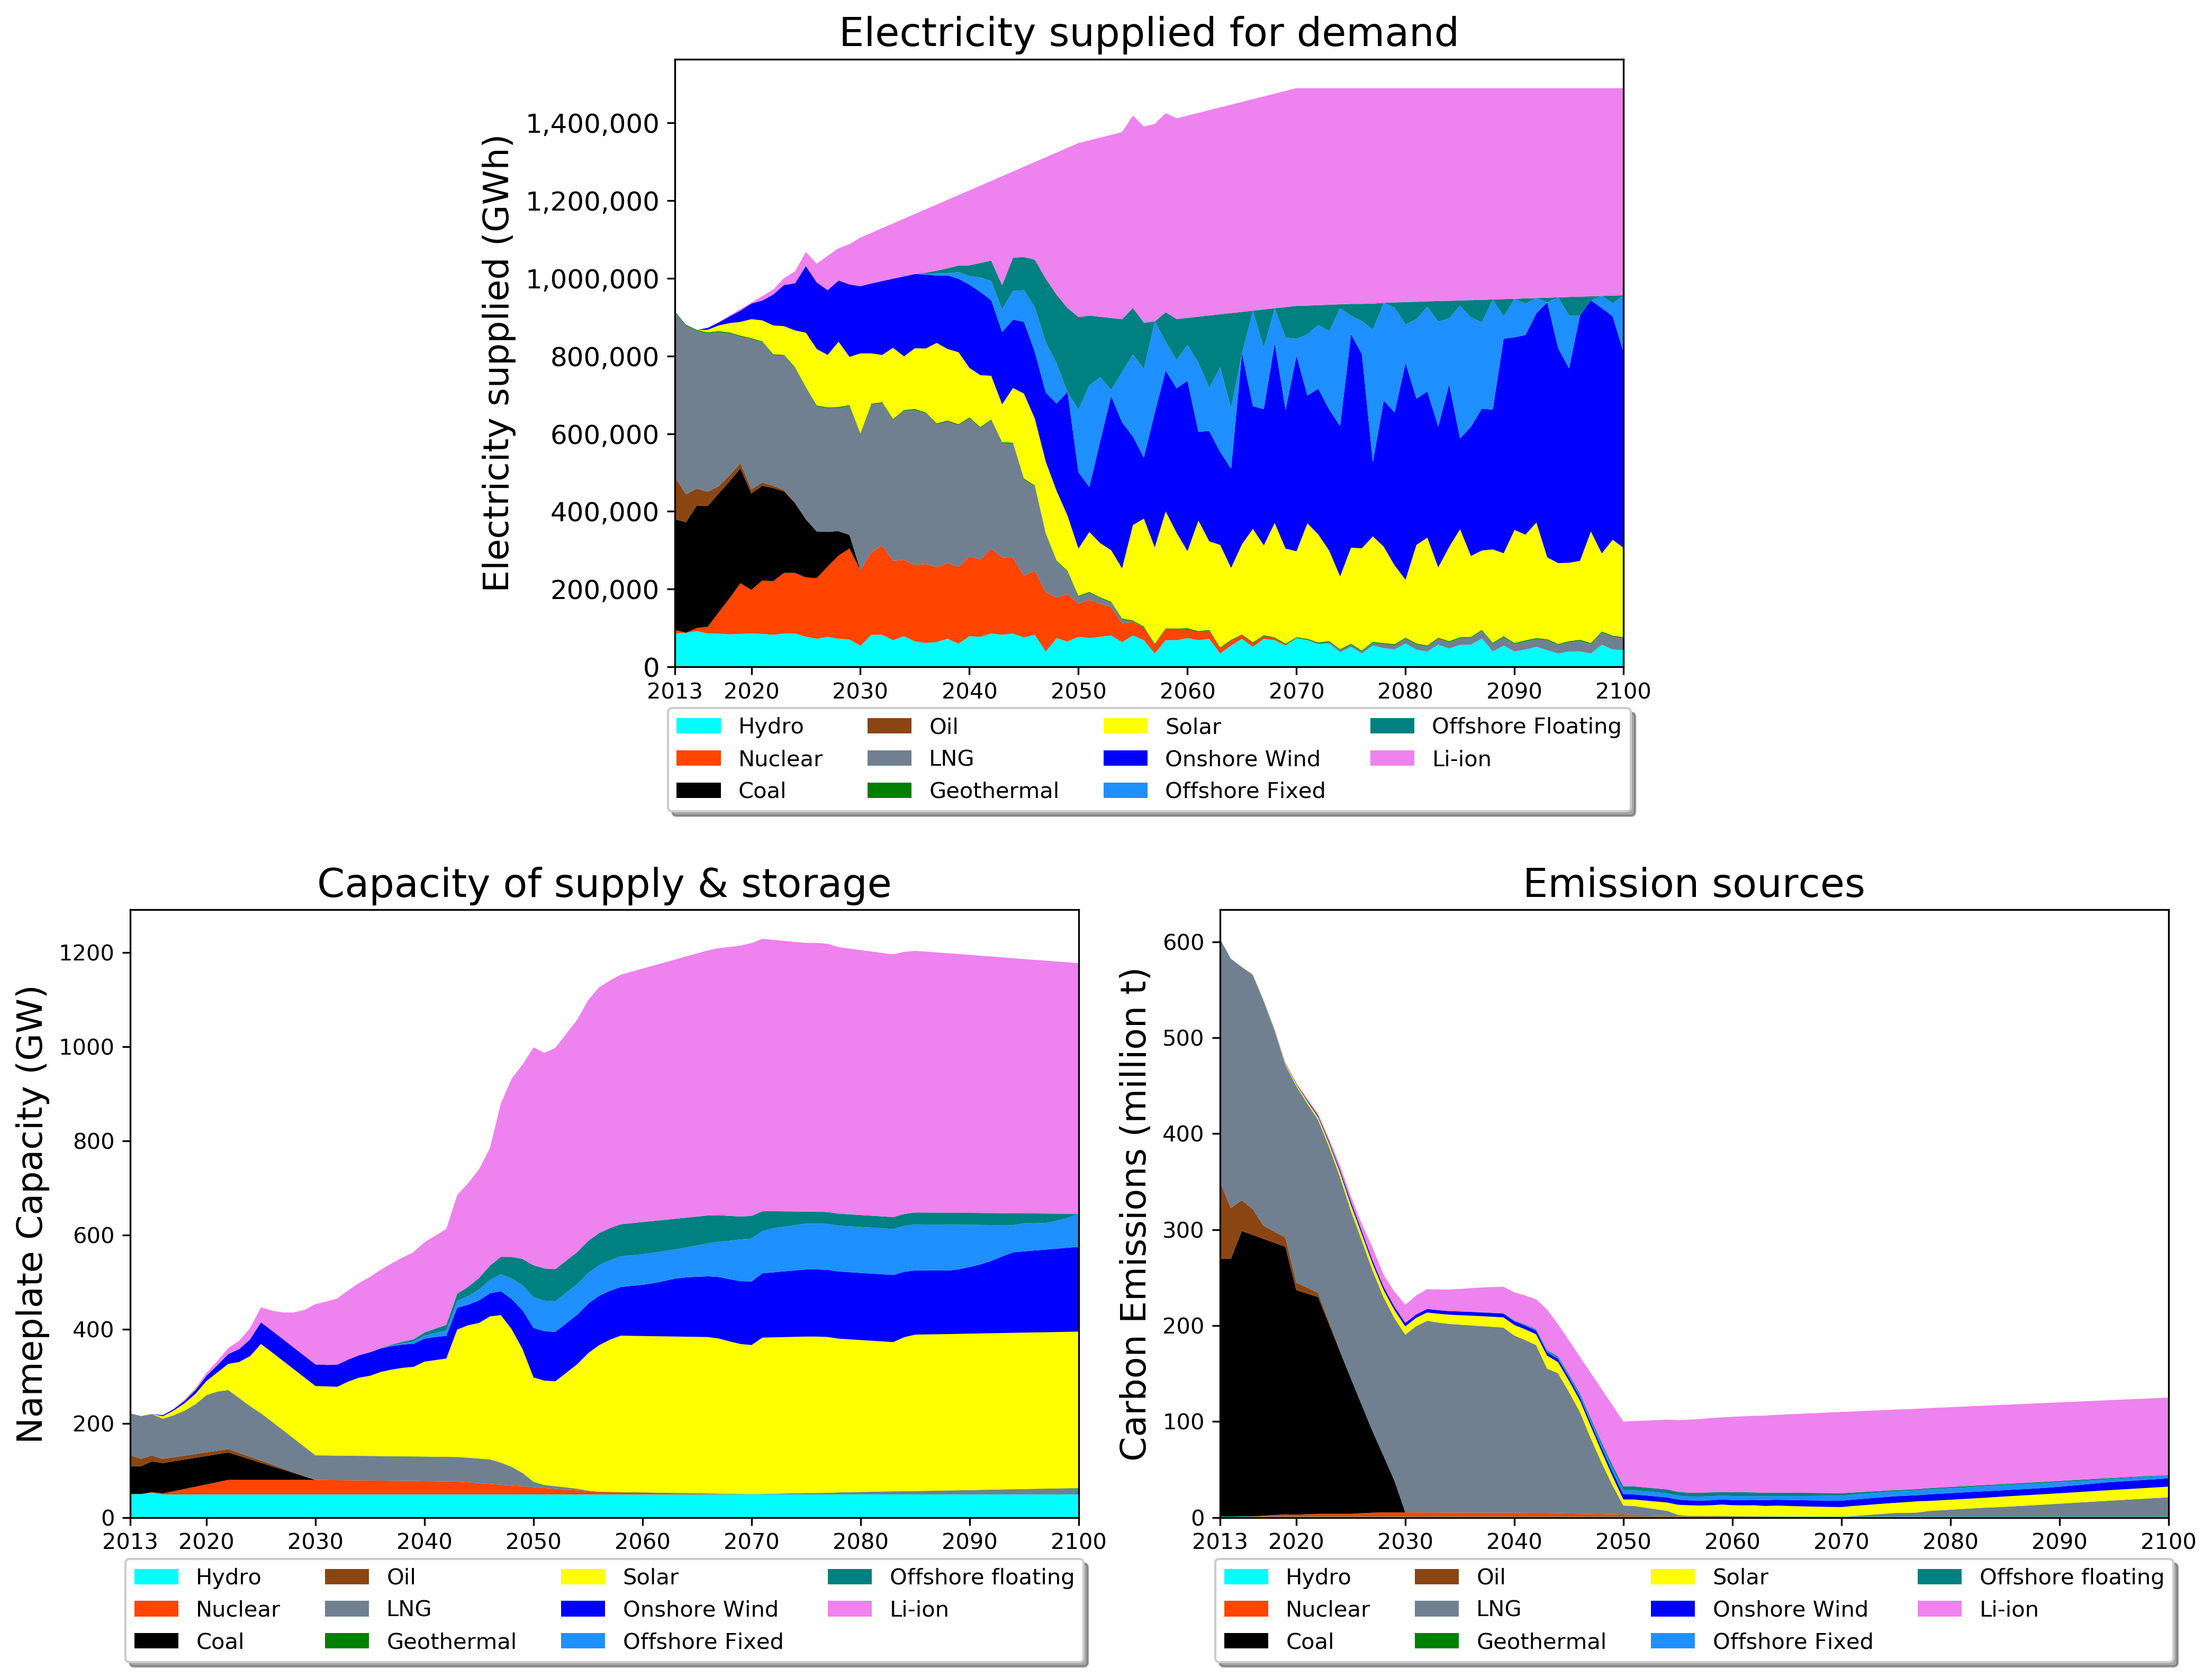
\includegraphics[scale=0.5]{figures/conv_nonuc}
\caption{Scenario 1 results (conventional technologies without new nuclear). The plot at the top shows the electricity generation mix used to meet the demand, the bottom-left figure shows the nameplate capacities of electricity generation and storage technologies that are deployed to meet the demand, and the bottom-right figure shows the sources of emission(direct and life cycle) resulting from this energy mix.}
\label{scen1}
\end{figure}

With the availability of new nuclear reactors in Scenario 2 (Figure \ref{scen2}), both 2030 and 2050 emission targets are achieved, and a further emission reduction of 12 Mt occurs by 2100. The model chooses to rapidly deploy nuclear power plants at the maximum allowed growth rate despite the high investment cost of nuclear due to its low life-cycle emissions. This nuclear-driven reduction in emissions allows natural gas power plants to operate until 2100. The share of renewables deployed during this transition reduces dramatically. This, combined with the load-following capabilities of natural gas plants and nuclear reactors, drastically decreases the capacity of lithium-ion storage deployed. 12,220 TWh of electricity is diverted to storage, primarily from nuclear (46\%), solar (41\%), and onshore wind (8\%). The total transition cost of this scenario is the lowest, at \textbf{2.66 trillion USD.}

\begin{figure}[H] 
\centering
%\vspace*{-3cm}
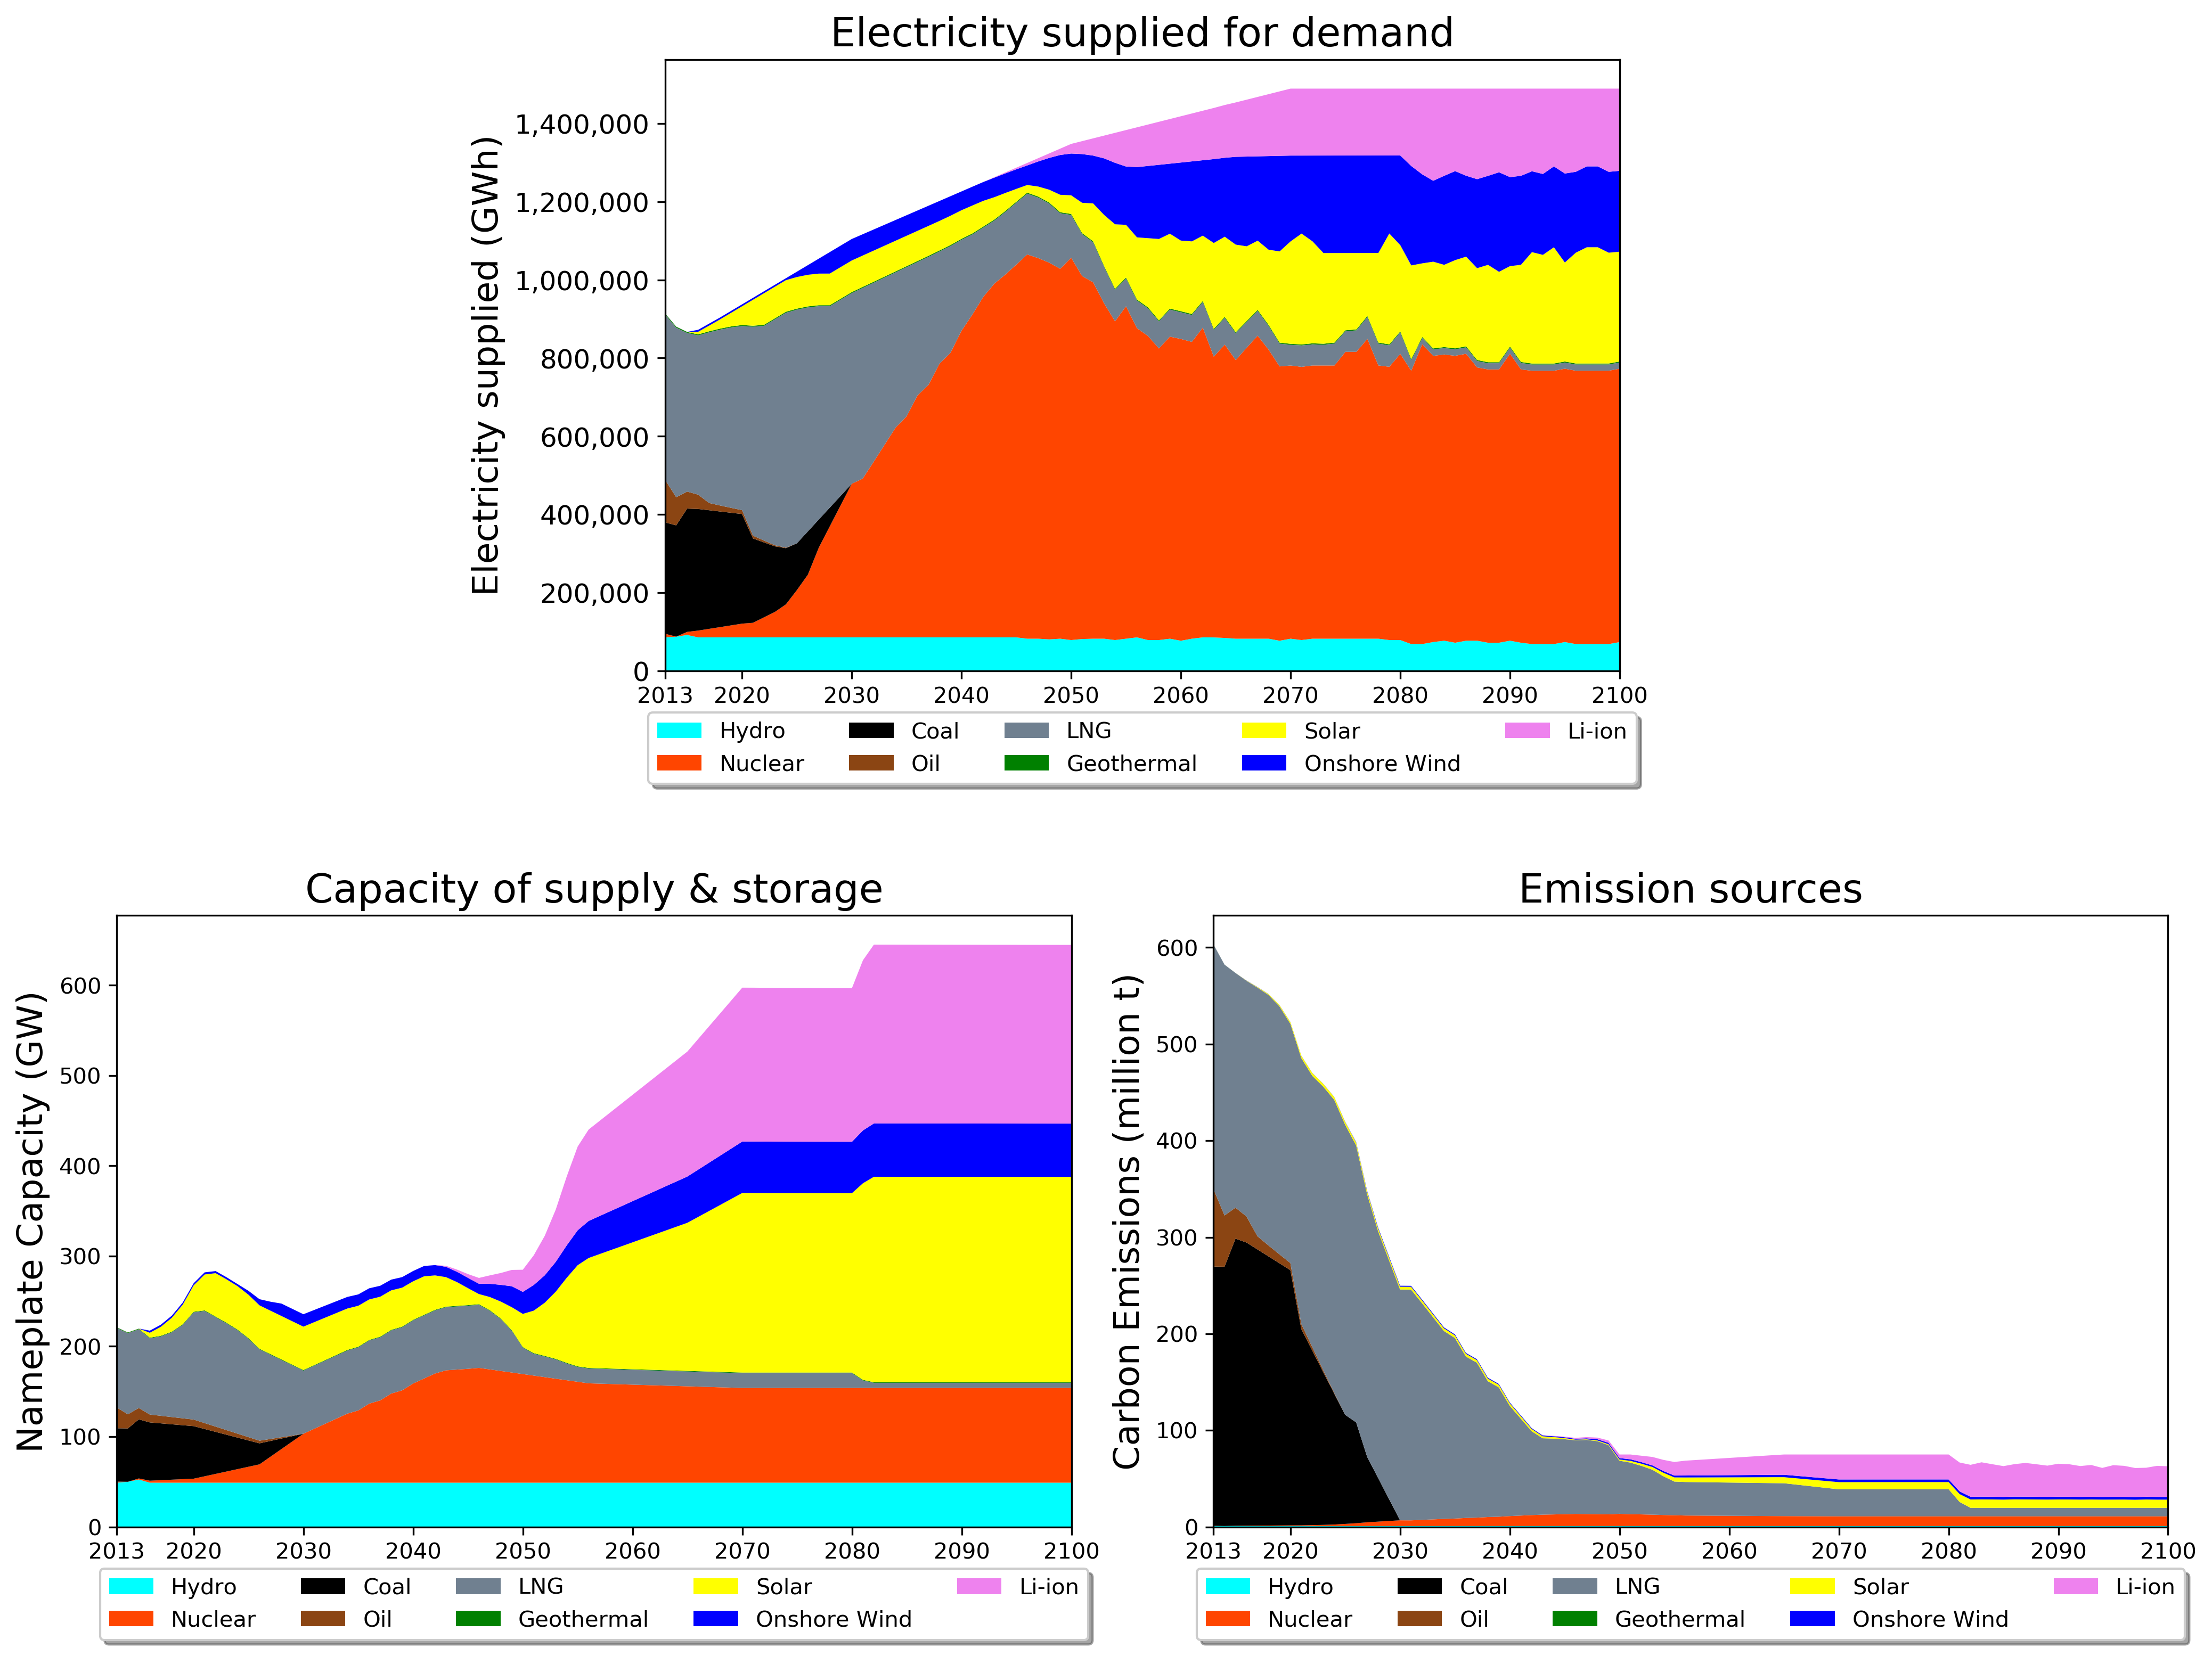
\includegraphics[scale=0.5]{figures/conv_nuc}
\caption{Scenario 2 results (conventional technologies with new nuclear). The plot at the top shows the electricity generation mix used to meet the demand, the bottom-left figure shows the nameplate capacities of electricity generation and storage technologies that are deployed to meet the demand, and the bottom-right figure shows the sources of emission(direct and life cycle) resulting from this energy mix.}
\label{scen2}
\end{figure}

Using emerging technologies without new nuclear power (Figure \ref{scen3}), the model is able to meet both the 2030 and 2050 emission reduction goals, but no further decarbonisation occurs after 2050. The results highlight the need to restart Japan's existing nuclear power plants at full capacity by 2030 in such a scenario. The deep emission cuts achieved through renewables, hydrogen, and \gls{CCS} allow the model to keep using \gls{lng} until 2100. Expansion of solar and onshore wind, along with a modest deployment of lithium-ion batteries and natural gas with \gls{CCS}, helps the model meet 2030 emission goals. After that, the model relies primarily on renewables and hydrogen to curb emissions. Rapid investment in hydrogen storage from 2030 onwards allows effective utilisation of renewables and precludes investment in offshore floating wind power. \gls{lng}-based \gls{CCS} plays a modest role as an intermediate technology before the model can complete the transition to utility-scale hydrogen. Between 2032-2077, the model generates 2,328 TWh  of electricity from \gls{CCS} technology, which is 2\% of the electricity generated over the entire simulation time frame. This results in 872 Mt of CO$_2$ being captured, which is well within the estimated 156 Gt CO$_2$ reservoir limit for Japan \cite{kato_energy_2016}. As the existing photovoltaic technology approaches the end of its lifetime and emerging solar technologies become cheaper and more efficient, they rapidly replace existing solar power, benefiting from the existing solar manufacture and supply chains. A total of 43,879 TWh of generated electricity is diverted to storage, primarily from solar and emerging solar technologies (48\%), fixed bottom offshore wind (28\%), and onshore wind (20\%). Much of this is used to generate 35,478 TWh worth of hydrogen, initially from alkaline electrolysis(1\%), but rapidly transitioning to PEM electrolysis (99\%) due to its greater efficiency and increasing cost-effectiveness. The cost of this transition is \textbf{3.19 trillion USD}.

\begin{figure}[H] 
\centering
%\vspace*{-3cm}
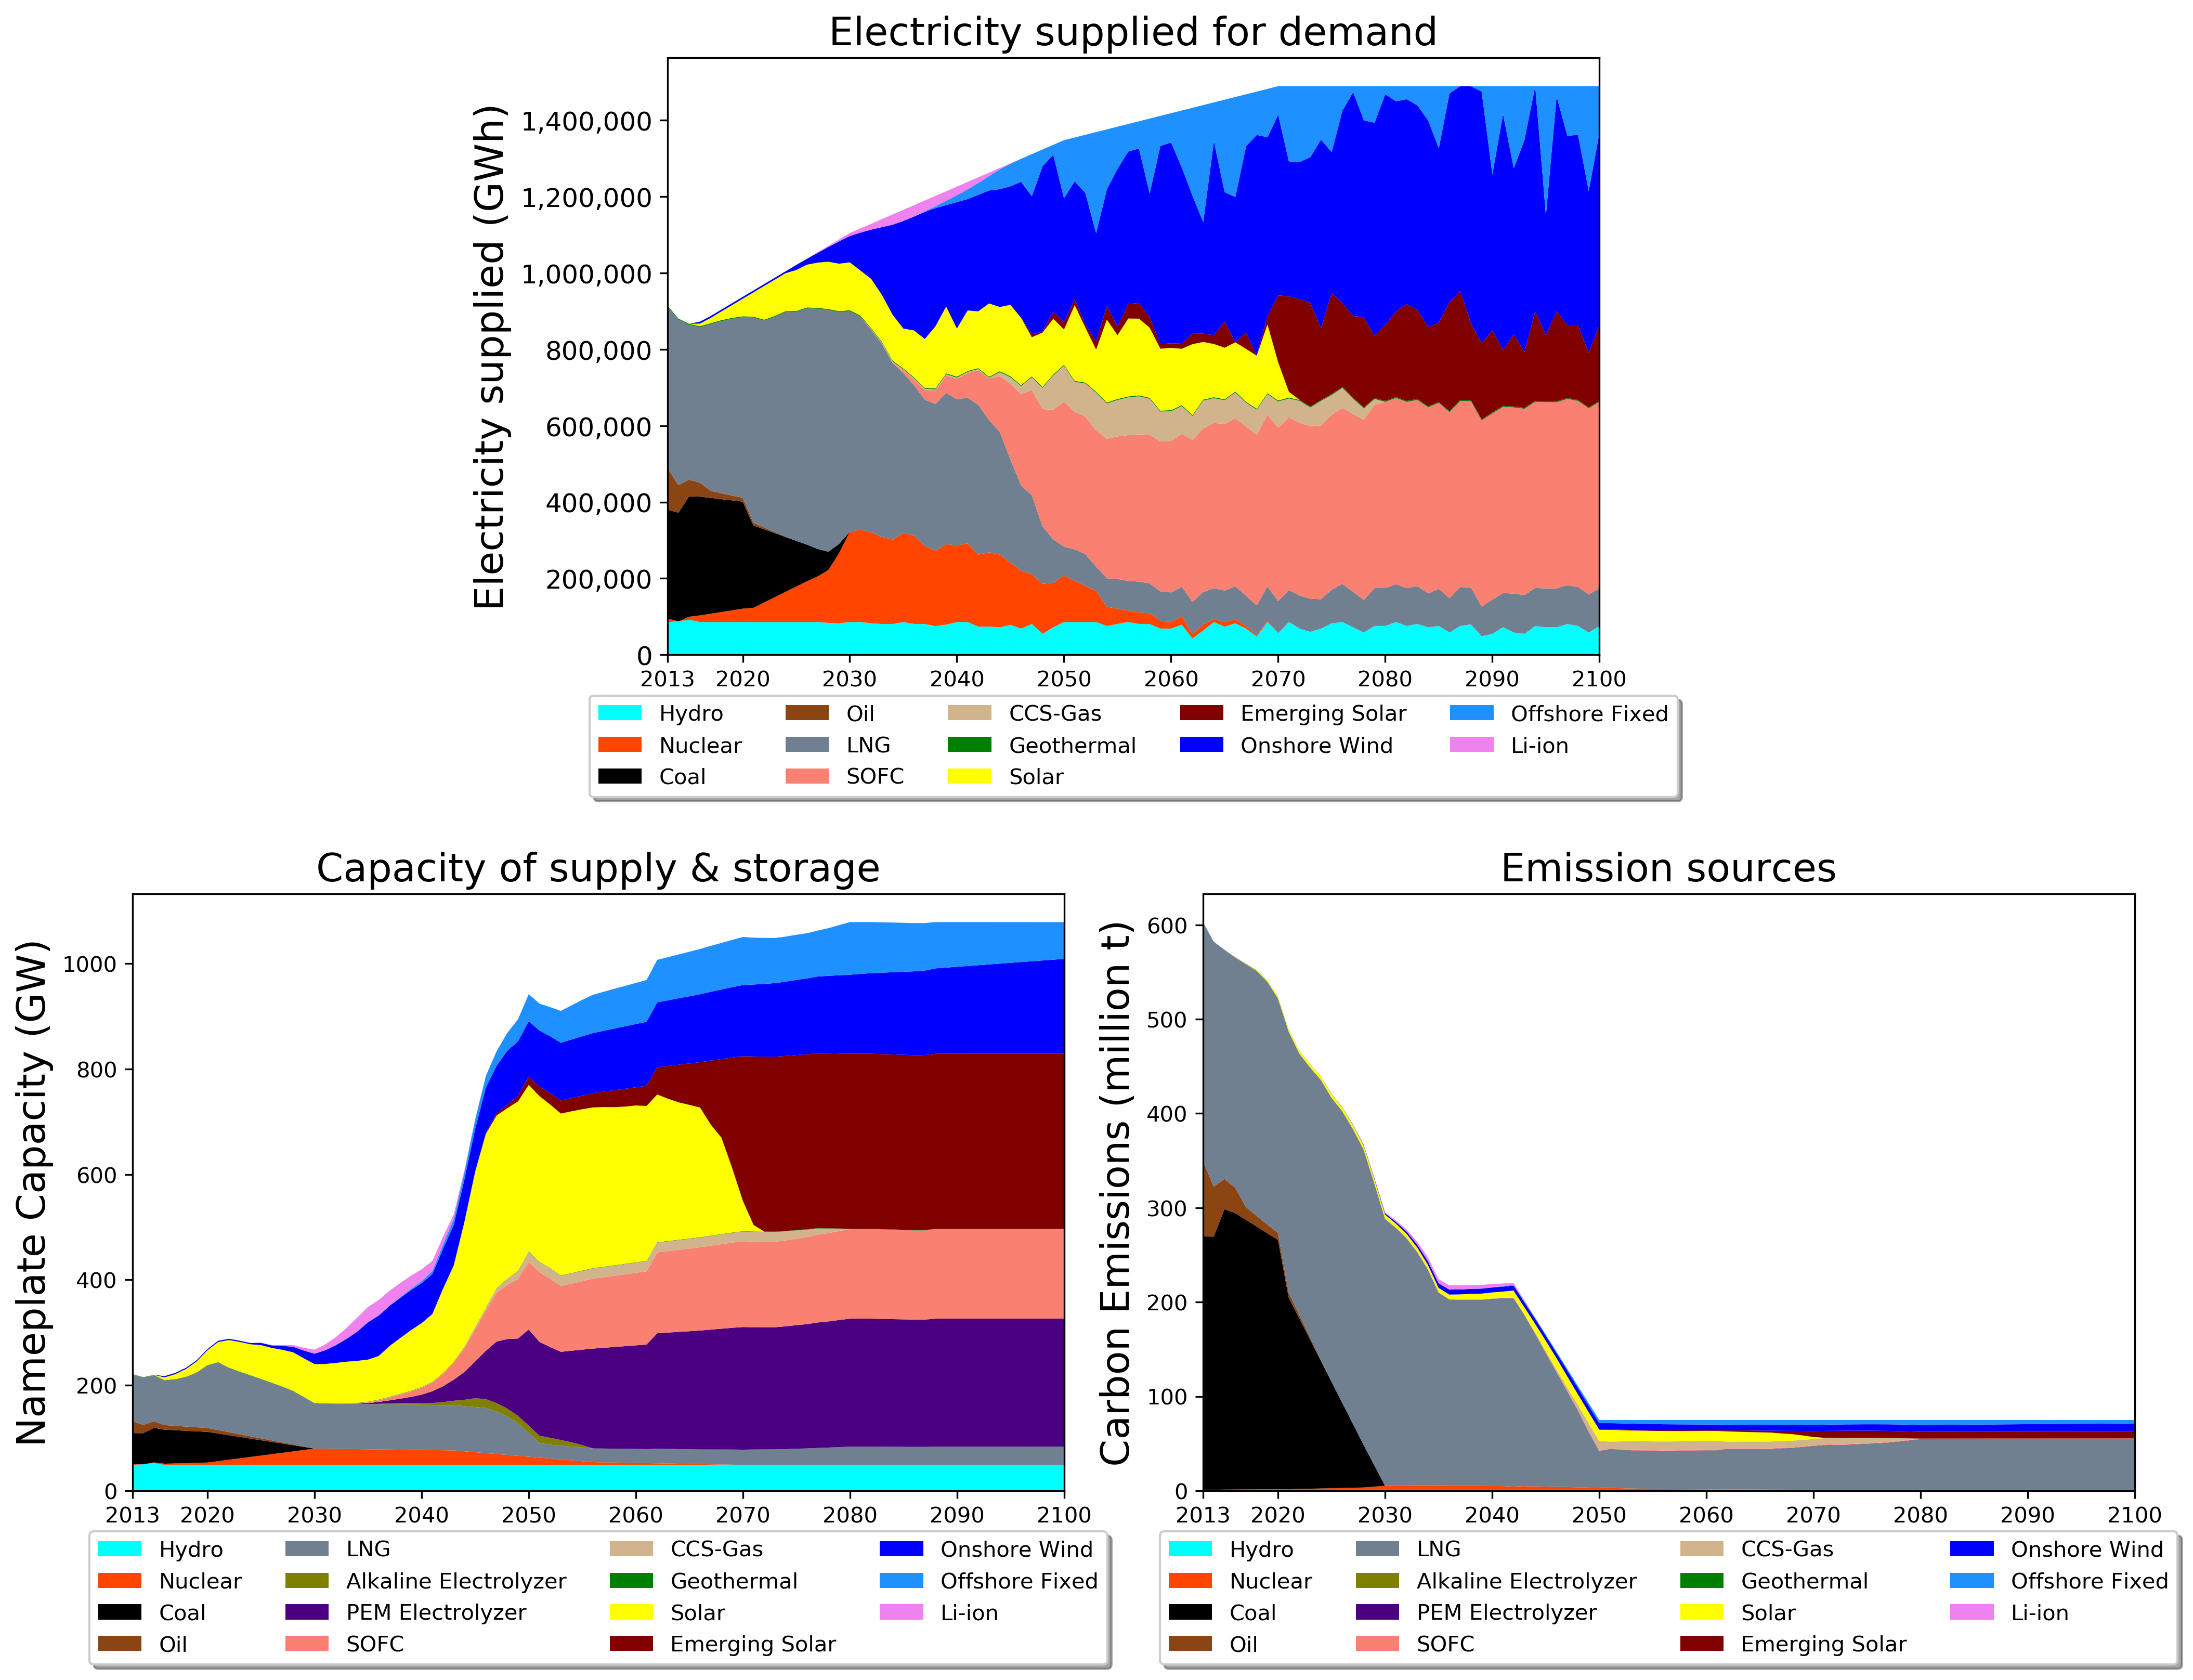
\includegraphics[scale=0.5]{figures/newtechs_nonuc}
\caption{Scenario 3 results (emerging technologies without new nuclear). The plot at the top shows the electricity generation mix used to meet the demand, the bottom-left figure shows the nameplate capacities of electricity generation and storage technologies that are deployed to meet the demand, and the bottom-right figure shows the sources of emission(direct and life cycle) resulting from this energy mix.}
\label{scen3}
\end{figure}

Deploying both emerging technologies with new nuclear reactors (Figure \ref{scen4}) results in rapid decarbonisation. Both 2030 and 2050 emission targets are met, and an additional emissions reduction of 32 Mt occurs by 2100. The deployment of 50 MW nuclear obviates the need to invest in offshore wind, lithium-ion storage, and \gls{CCS}. Hydrogen plays a significant role in decarbonisation, but it is deployed from 2035 onwards instead of 2030, as in Scenario 3. The amount of electricity diverted to storage technologies is 29,733 TWh, primarily from solar and emerging solar technologies (62\%), onshore wind (20\%), and nuclear (13\%). From this, 24,264 TWh of hydrogen is generated, produced entirely from PEM electrolysis, as there was no urgency to deploy \gls{AEC} as in Scenario 3. The cost of this transition is \textbf{2.80 trillion USD}.

\begin{figure}[H] 
\centering
%\vspace*{-3cm}
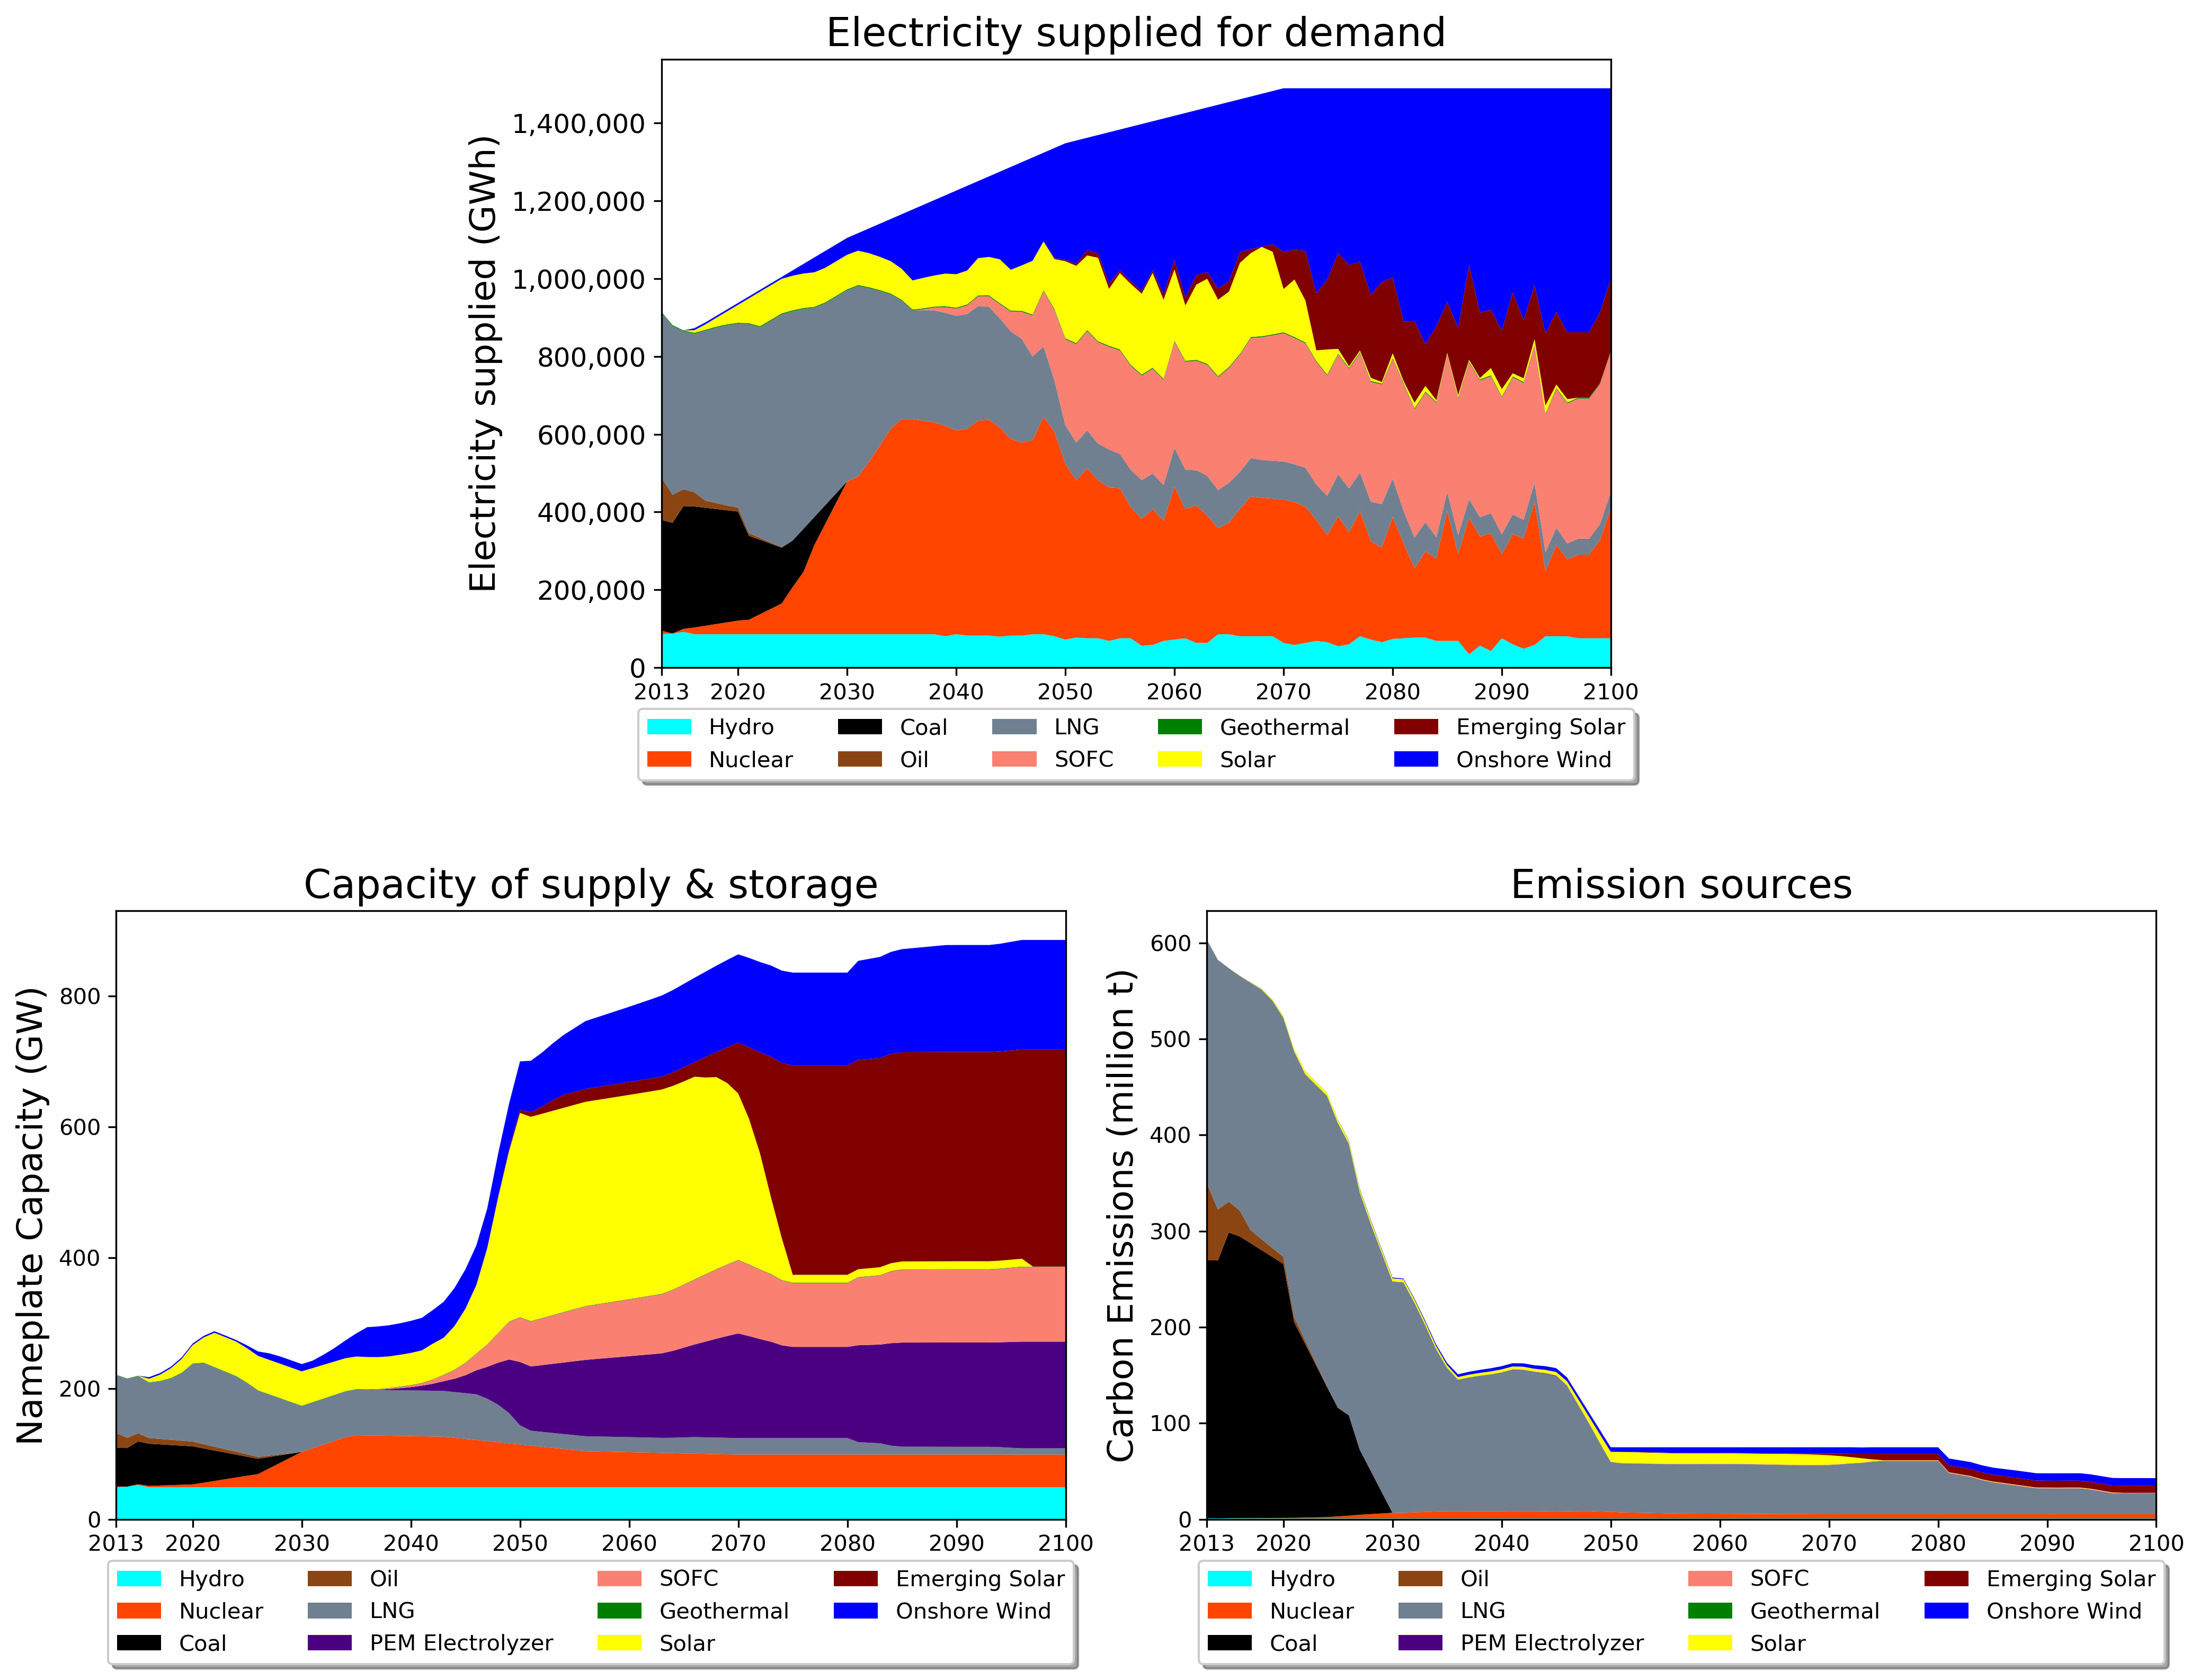
\includegraphics[scale=0.5]{figures/newtechs_nuc}
\caption{Scenario 4 results (emerging technologies with new nuclear). The plot at the top shows the electricity generation mix used to meet the demand, the bottom-left figure shows the nameplate capacities of electricity generation and storage technologies that are deployed to meet the demand, and the bottom-right figure shows the sources of emission(direct and life cycle) resulting from this energy mix.}
\label{scen4}
\end{figure}

The fifth scenario's results (Figure \ref{scen5}) closely resemble those of the third scenario (Figure \ref{scen3}). However, \gls{SOEC}s rapidly replace a large fraction of aging \gls{PEMEC}s, starting from 2055. Some \gls{PEMEC}s remain in the mix until 2100 despite their lower efficiency due to their lower cost. Both 2030 and 2050 emission targets are met, but no additional emission reductions occur beyond 2050. The amount of electricity diverted to storage technologies is 41,752 TWh, primarily from solar and emerging solar technologies (48\%), onshore wind (28\%), and fixed-bottom offshore wind (20\%). From this, 35,550 TWh of hydrogen is generated, mostly from \gls{SOEC} (56\%), and \gls{PEMEC} (43\%). \gls{AEC} contributes a mere 0.95\% of the total hydrogen, and \gls{PWS} plays the smallest role at 0.05\%. The cost of this transition is \textbf{3.18 trillion USD}.

\begin{figure}[H] 
\centering
%\vspace*{-3cm}
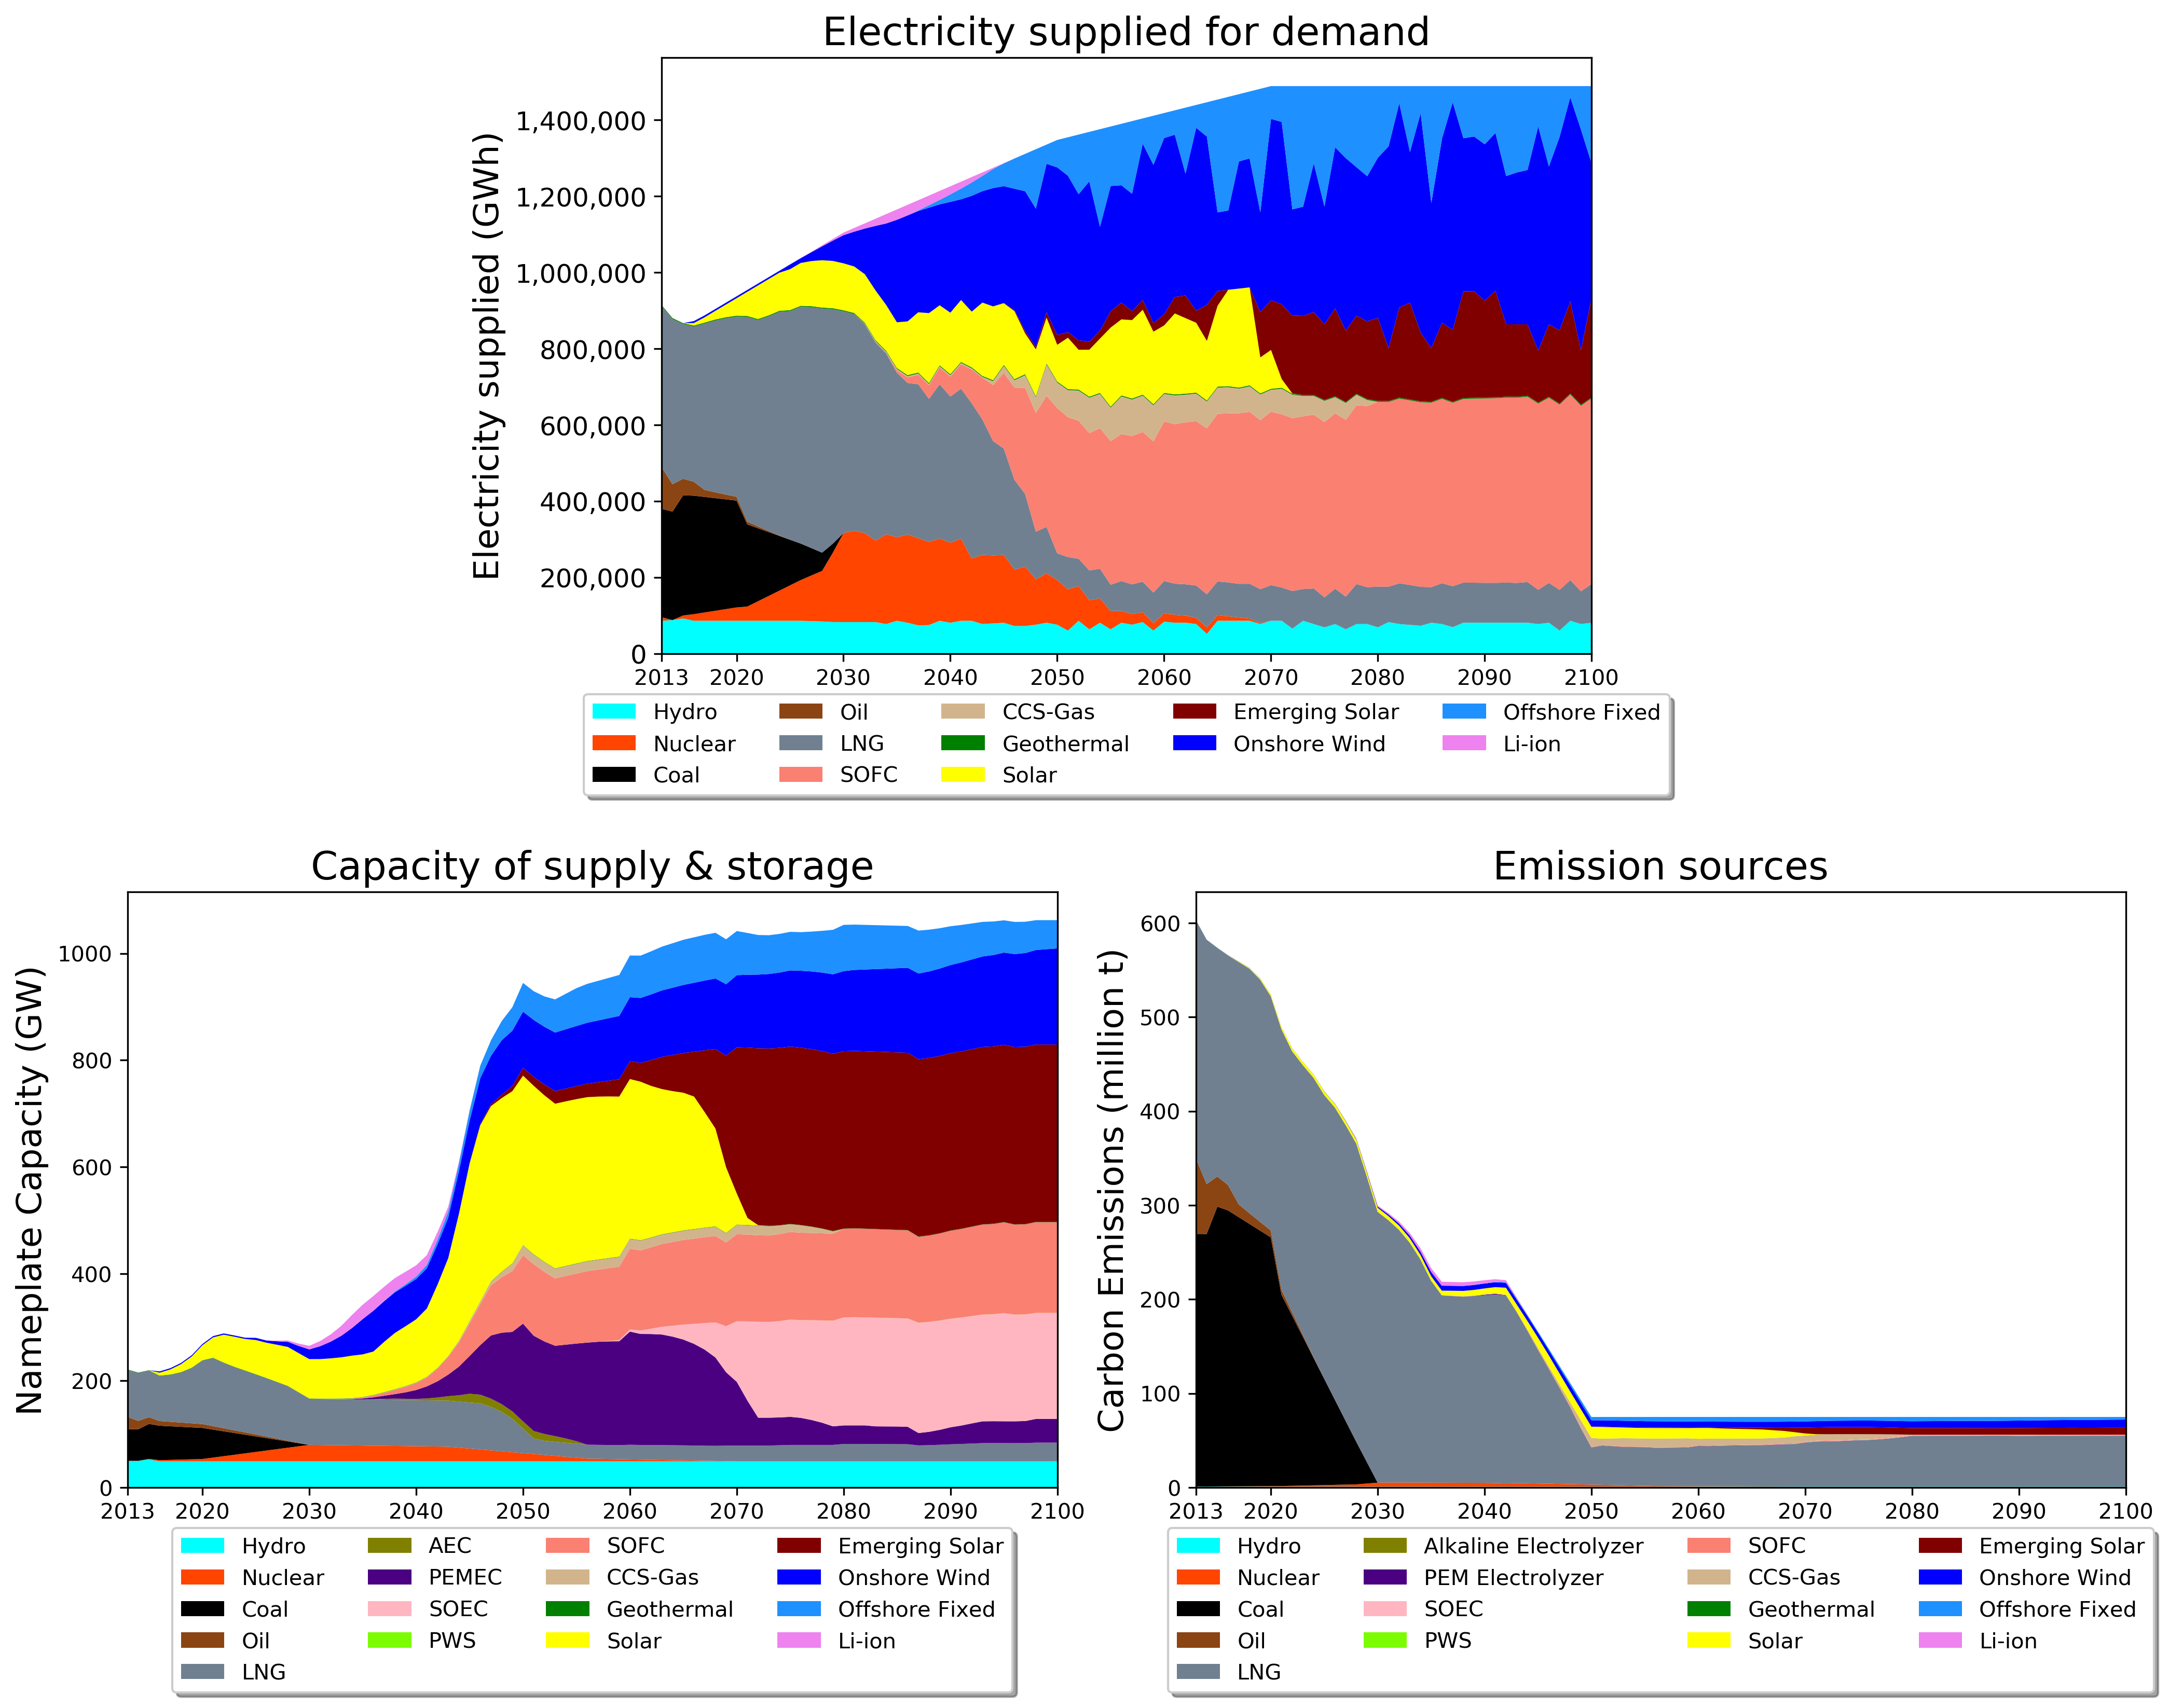
\includegraphics[scale=0.5]{figures/lowtrltech_nonuc}
\caption{Scenario 5 results (emerging technologies and nascent hydrogen technologies without new nuclear). The plot at the top shows the electricity generation mix used to meet the demand, the bottom-left figure shows the nameplate capacities of electricity generation and storage technologies that are deployed to meet the demand, and the bottom-right figure shows the sources of emission(direct and life cycle) resulting from this energy mix.}
\label{scen5}
\end{figure}

\subsection{Sensitivity analysis}

\begin{figure}[H] 
\centering
\hspace*{-1cm}
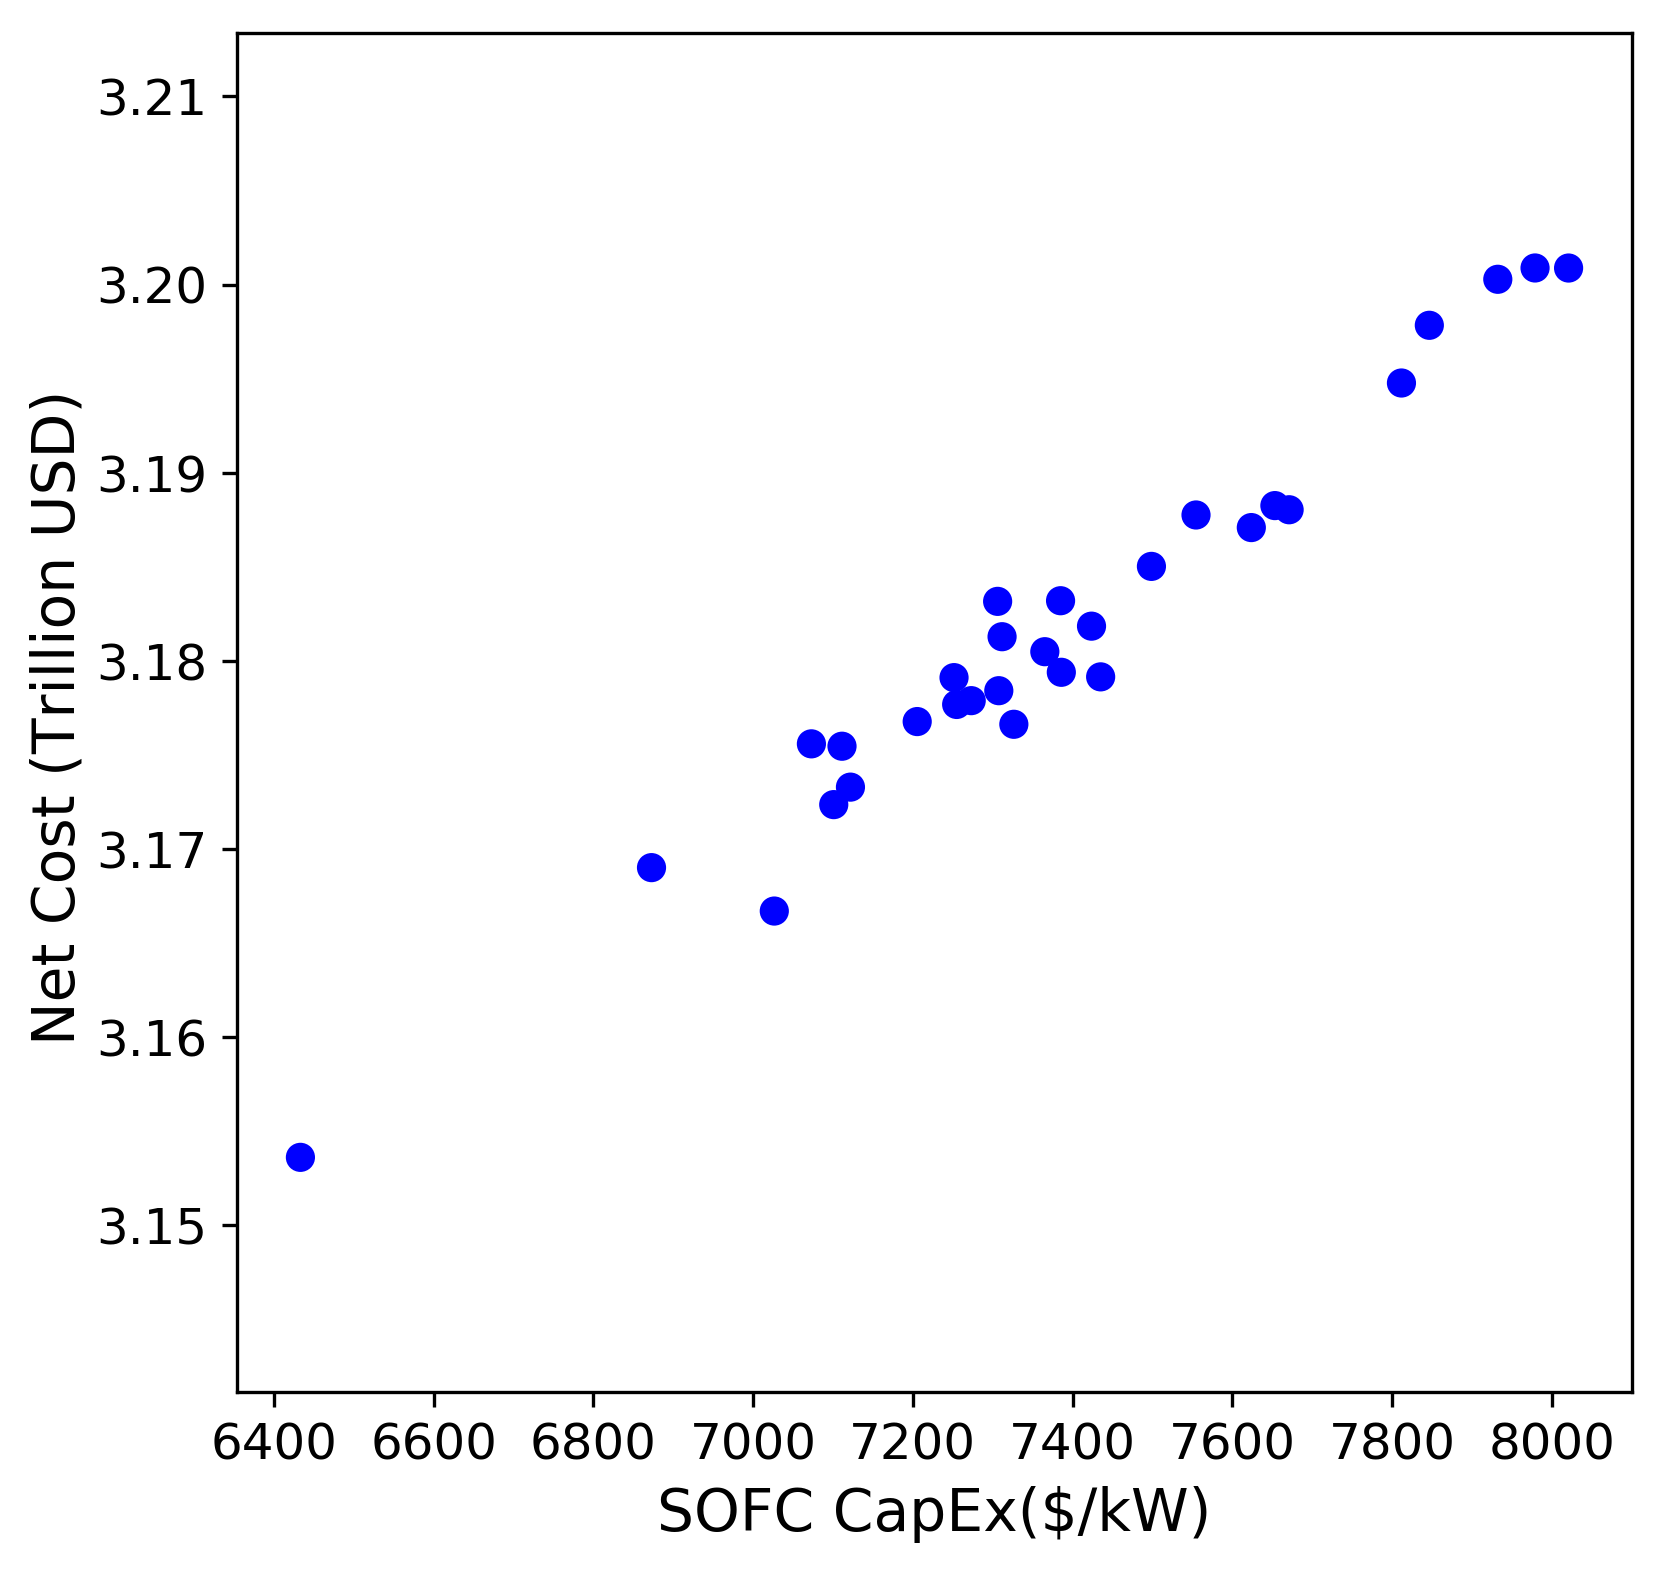
\includegraphics[scale=0.7]{figures/syscost_abbrv}
\caption{Sensitivity analysis for overall transition cost vs. solid oxide fuel cell capital costs.}
\label{syscost-smol}
\end{figure}

\begin{figure}[H] 
\centering
%\hspace*{-3cm}
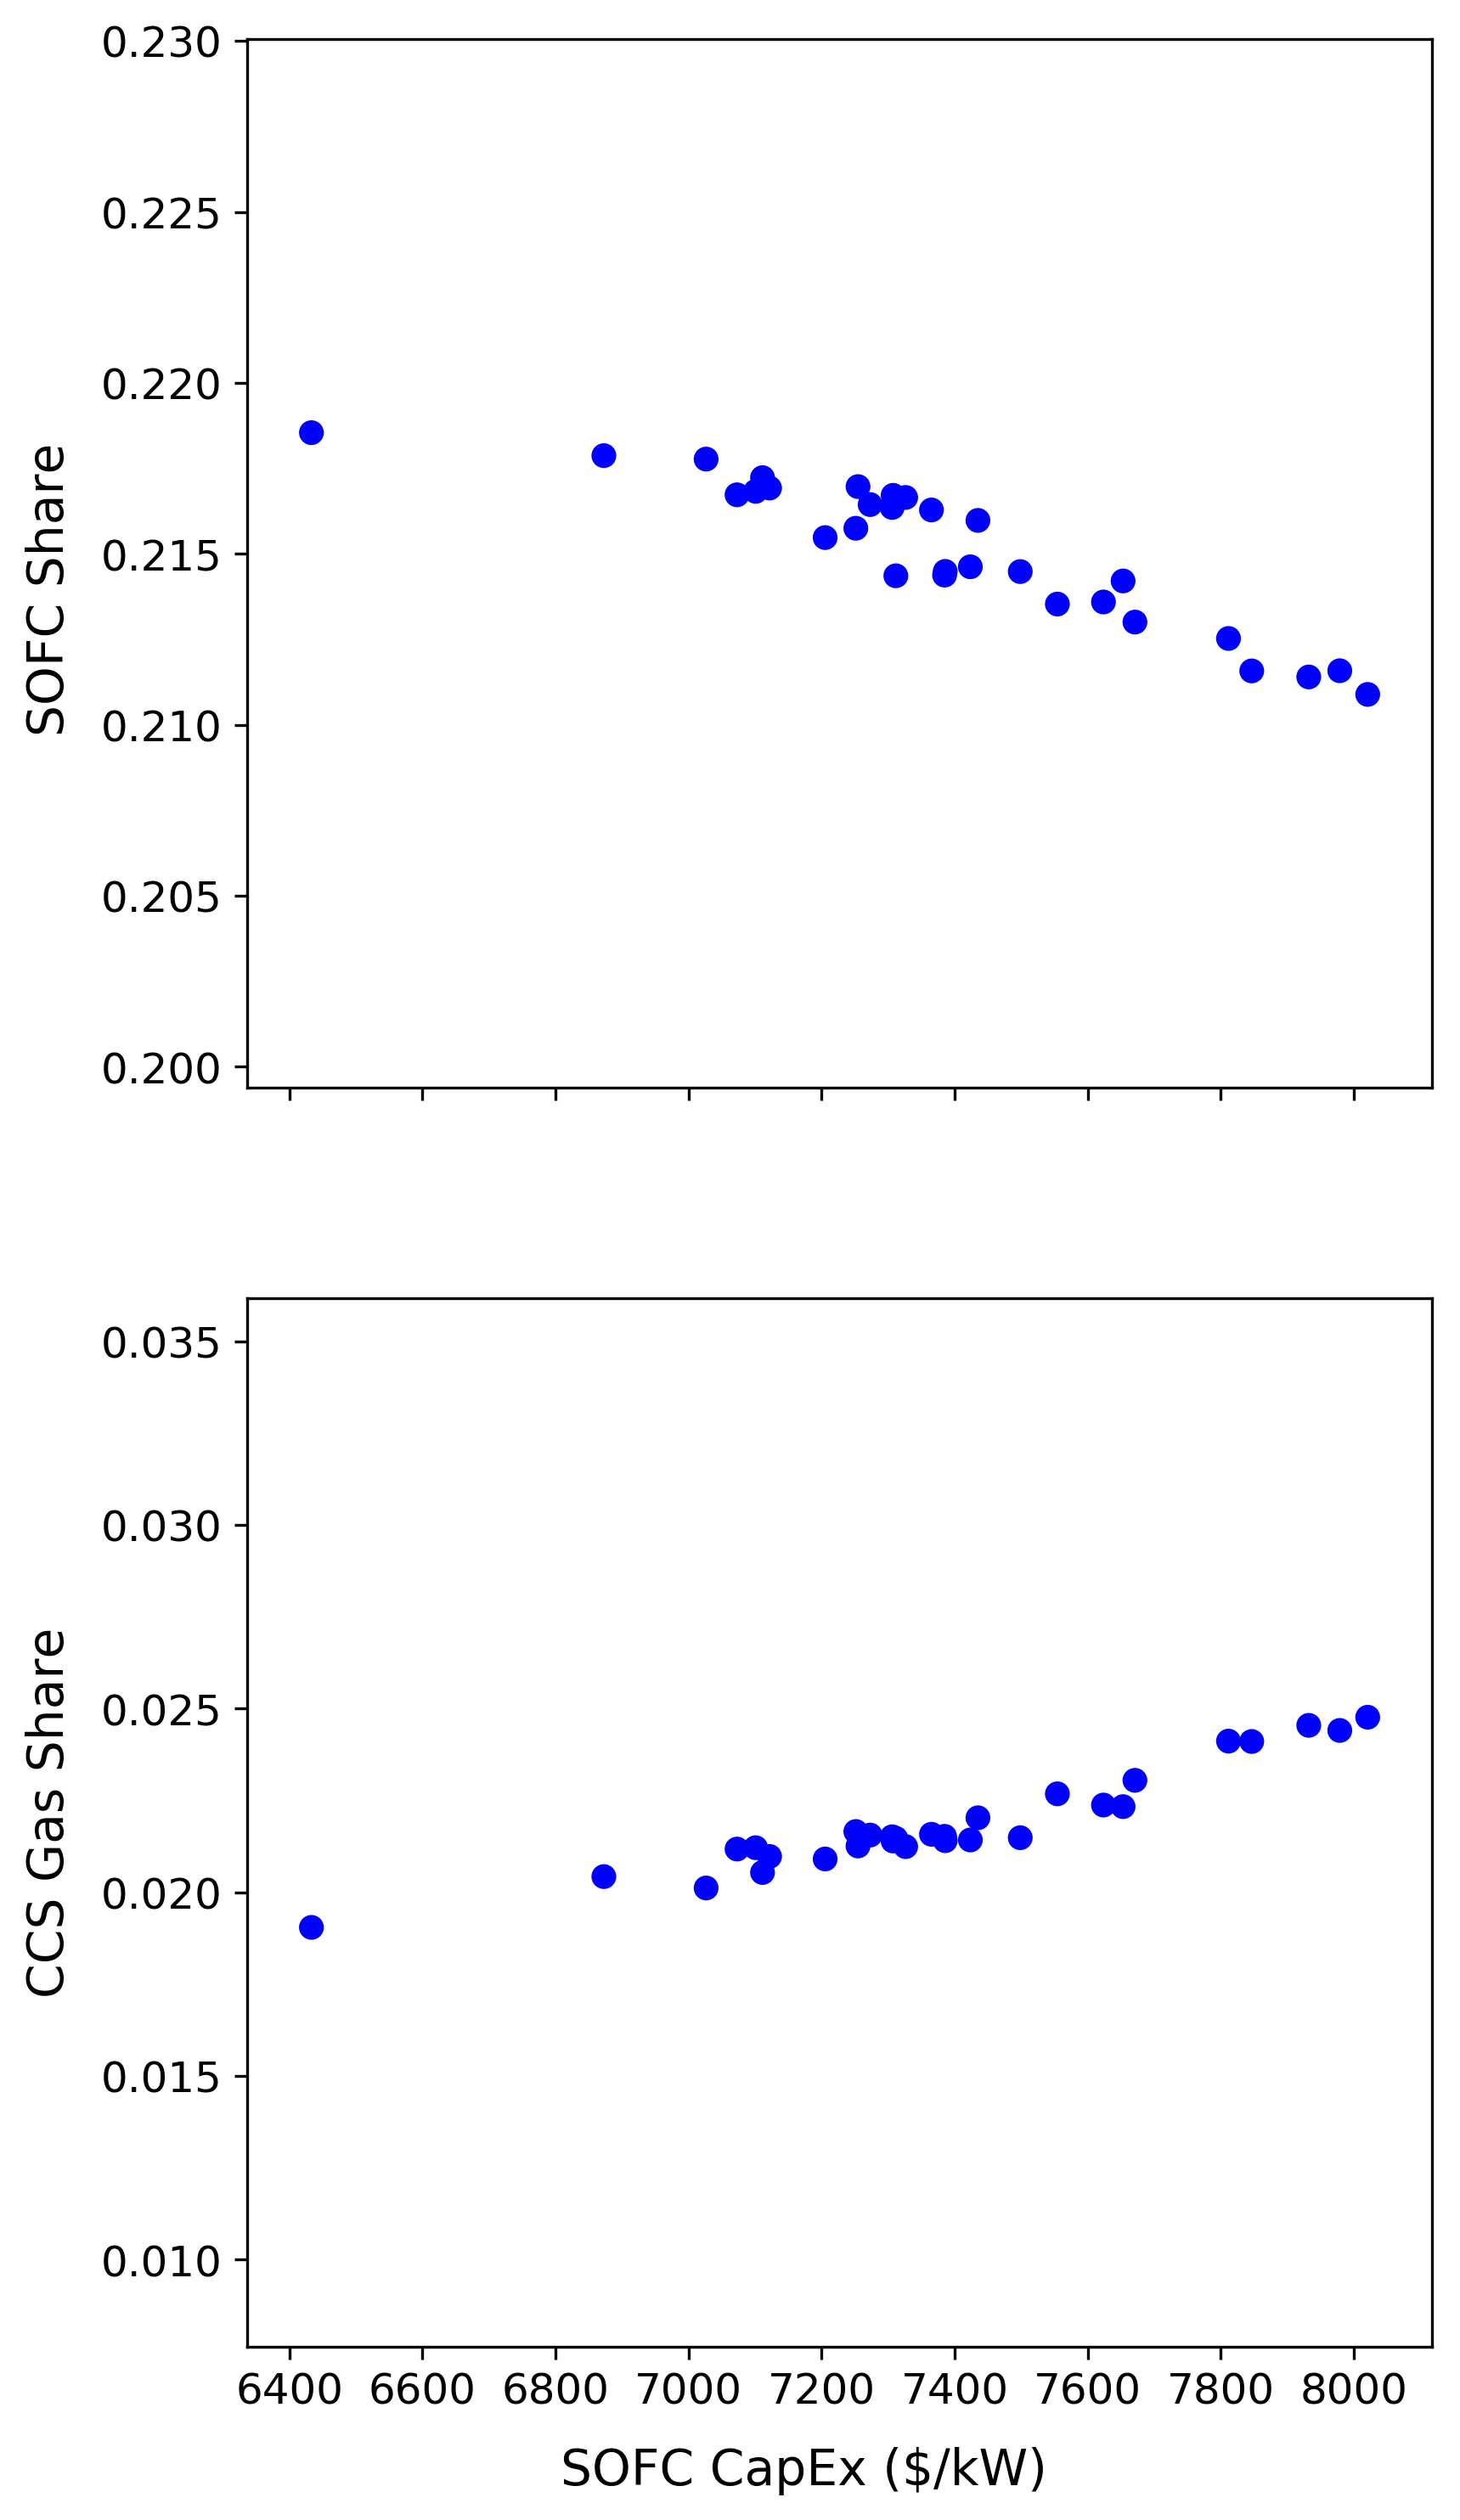
\includegraphics[scale=0.7]{figures/satechselc_abbrv}
\caption{Sensitivity analysis results for electricity supply shares of solid oxide fuel cells (top) and carbon capture and sequestration natural gas plants (bottom) vs solid oxide fuel cell capital costs.}
\label{satechs-smol}
\end{figure}

Results from our sensitivity analysis are partially presented in Figures \ref{syscost-smol} and \ref{satechs-smol}, whereas the complete results are in in the appendix (Figs. \ref{pws}-\ref{sa-useless}). The overall transition cost is strongly correlated with the investment cost of \gls{SOFC}s (Figure \ref{satechs-smol}). This follows from the large share of \gls{SOFC}s, as they are the most important low-carbon technology for storing renewable power, yet they are the most expensive technology available to the model. In the absence of new nuclear deployments, \glspl{SOFC} are irreplaceable, and their share is largely fixed. In analysing the sensitivity of the output of electricity generation technologies (Figure \ref{satechs-smol}), we unsurprisingly found the output of \gls{SOFC}s most strongly correlated with their own capital costs. However, the output of \gls{CCS} with natural gas was also most strongly correlated with the investment cost of \gls{SOFC}s, rather than the investment cost of CCS gas itself. The share of \gls{CCS} with natural gas is also relatively small (indicated by the y-values in Figure \ref{satechs-smol}), about 2-3\%.  This is because CCS gas deployment increases only marginally as fuel cells deployment decreases due to increasing fuel cell cost. Therefore, the role of CCS with natural gas is that of a secondary stopgap technology that is deployed when other decarbonisation alternatives are uneconomical. This is due to the large life-cycle and direct emissions of CCS gas compared to renewables and hydrogen technologies.

Remaining results indicate that \gls{PEMFC}s are never utilised because of their low efficiency compared to \gls{SOFC}s, and \gls{CCS} coal plants are never deployed due to their high emission coefficient (Figure \ref{sa-useless}). \gls{PWS} plays a minor role in generating 0-20 TWh of hydrogen over the entire simulation's time-period (Figure \ref{pws}), as opposed to \gls{SOEC}s which generate 19,500-22,500 TWh, and \gls{PEMEC}s, which generate 12,000-16,000 TWh of hydrogen, respectively. The share of \gls{PWS} was found to be strongly correlated with its investment cost, with \$3300/kW the approximate threshold at which this technology ceases to be cost-competitive (Figure \ref{pws}). \gls{PWS} deployment is also weakly correlated with the splitting efficiency; values over 21\% seem most favourable. The \gls{PWS} emission coefficient is too small to have an impact on the overall emissions of the system considering \gls{PWS}'s small deployment. Hence its emission coefficient does not appreciably affect \gls{PWS} deployment. Since \gls{PEMFC}s, \gls{CCS} coal, and \gls{PWS} are not deployed in quantities significant enough to affect the model's performance, they are omitted as potential dependent variables for the rest of the sensitivity analysis.

For hydrogen generating technologies (Figure \ref{satechs-h2}), the \gls{SOEC} output is most strongly correlated with the SOEC investment cost. However, \gls{SOEC} output is affected insignificantly by the perturbation applied to its investment cost. \gls{SOEC} deployment is largely insensitive to its emission coefficient as its contribution to overall emissions is negligible. This highlights \gls{SOEC}'s vital role in the transition. \gls{PEMEC} (Figure \ref{satechs-elc}) deployment is also most noticeably affected by its respective investment costs, but also by the investment cost of SOECs - as SOECs become more expensive, \gls{PEMEC}s emerge as the natural replacement.